% This is samplepaper.tex, a sample chapter demonstrating the
% LLNCS macro package for Springer Computer Science proceedings;
% Version 2.20 of 2017/10/04
%
\documentclass[runningheads]{llncs}
%
\usepackage{graphicx}
\usepackage{caption}
\usepackage[dvipsnames]{xcolor}
% Used for displaying a sample figure. If possible, figure files should
% be included in EPS format.
%
% If you use the hyperref package, please uncomment the following line
% to display URLs in blue roman font according to Springer's eBook style:
% \usepackage{hyperref}
% \renewcommand\UrlFont{\color{blue}\rmfamily}

\begin{document}
%
\title{PNG-Fuzzing with JQF}
%
%\titlerunning{Abbreviated paper title}
% If the paper title is too long for the running head, you can set
% an abbreviated paper title here
%
\author{Paul Kalz \and Marwin Linke \and Sebastian Schatz}
%
\institute{Humboldt University of Berlin, Germany}
\maketitle              % typeset the header of the contribution
%
\begin{abstract}
Fuzzing is a dynamic testing technique used to discover bugs and
security issues in programmes and software systems. It is an essential
technique of software testing and security assurance. There are different
fuzzing strategies ranging from simple mutation-based techniques to more
advanced generator-based techniques, but they all have in common that
they operate by automatically injecting a lot of different data into a target
program's inputs to uncover bugs, unforeseen behaviors, system failures or
vulnerabilities.

The paper aims to summarize programming of a generator-based PNG fuzzer
in JQF, with the target library of our fuzzer being PNGJ. Firstly, the paper
provides a brief overview of the concept of usage of PNG and its
specifications, as well as the security of PNG files. Furthermore, an overview
regarding used tools and the process, had been provided. The
implementation of the PNG generator is shown in detail and an overview of
the implementation of the fuzz driver has been provided. Finally, the paper
provides evaluation and discussion of the results.
Keywords: PNG, Fuzzer, JQF

\keywords{PNG  \and Fuzzing \and JQF.}
\end{abstract}
%
%
%
\section{Background on the File Format PNG}
\subsection{Overview}
%TODO: Overview: Gebt einen kurzen Überblick über das ausgewählte Datenformat (Historie, Verwendungszweck,...)

\subsubsection{History}
The idea of PNG and its development started in January 1995 after the
compression algorithm LZW, used in GIF (Graphics Interchange Format), was
patented. Authors of GIF-supporting software had to pay to use it since
December 1994. PNG stands for Portable Network Graphics and was designed to be better, smaller
and more extensible than GIF. PNG is free and supposed to be the successor of
GIF.

On the 1st of October 1996, PNG spec 1.0 was approved as W3C
Recommendation and on the 15th of January 1997, PNG spec 1.0 was released as
Informational RFC 2083 (IETF)~\cite{PNG_specification}. In 2004, PNG was published as an ISO/IEC 15948
standard.

\subsubsection{Use Cases}
PNG is a raster-graphics file format, which allows lossless data compression and
supports RGB and RGBA colors, as well as grayscale images. At default PNG does not allow
animated graphics and is mostly used on the Internet for transferring images and
pictures, for example it is often used for icons and buttons on websites.
Since PNG does not support other color spaces than RGB/RGBA, it is not used for
professional-quality print graphics or professional photographs.

\subsection{Input Specification}
%TODO: Input Specification: Beschreibt im Detail die Spezifikation des Dateiformats. Wie sind Dateien dieses Formats aufgebaut? Existiert eine formale Spezifikation? Wie ist eine Beispieldatei aufgebaut?
PNG is specified as an Informational RFC 2083 (IETF) and has a formal specification as
an ISO/IEC 15948 standard.
This section provides a brief overview of the structure of PNG, more details are in
section \ref{generator} Generator. Based on the structure of PNG, its byte streams can be broken
down into chunks. There are different types of chunks with different information in
them~\cite{libpng_chunks}. 3 types of chunks are critical for every PNG: \texttt{IHDR}, \texttt{IDAT} and \texttt{IEND}, that means
that they have to appear. There is another chunk that is critical for color type 3 called
\texttt{PLTE}. Every PNG file starts with the 8-byte signature \texttt{89 50 4E 47 0D 0A 1A 0A};
and each byte has its own purpose~\cite{libpng_rationale}.

\subsubsection{Example}
An example for a very small PNG image, displaying a single red pixel, is the following sequence of bytes:

\begin{center}
    \texttt{\color{NavyBlue}89 50 4E 47 0D 0A \color{PineGreen}1A 0A 00 00 00 0D 49 48 44 52 00 00 00 01 00 00 00 01 08 02
00 00 00 90 77 53 \color{Violet}DE 00 00 00 0C 49 44 41 54 08 D7 63 F8 CF C0 0000 03 01 01 00
18 DD 8D B0 \color{Plum}00 00 00 00 49 45 4E 44 AE 42 60 82}

\texttt{\color{NavyBlue}PNG \color{PineGreen}IHDR \color{Violet}IDAT \color{Plum}IEND}
\end{center}


\paragraph{Signature}
\begin{itemize}
    \item \texttt{{\color{NavyBlue}89}} distinguishes PNG files on systems that expect the first two bytes to identify the file type uniquely.
    \item \texttt{{\color{NavyBlue}50 4E 47}} stands for PNG in ASCII, so that if a person opens a PNG file in a text editor the first word is PNG.
    \item \texttt{{\color{NavyBlue}0D 0A}} catches bad file transfers that alter newline sequences.
    \item \texttt{{\color{NavyBlue}1A}} is a byte that stops the display of the file with DOS.
    \item \texttt{{\color{NavyBlue}0A}} checks for the inverse of the CR-LF translation problem.

\end{itemize}

\paragraph{Image Header (\texttt{IHDR})}
\begin{itemize}
    \item \texttt{\color{PineGreen}00 00 00 0D} This chunk has 13 bytes of content.
    \item \texttt{\color{PineGreen}49 48 44 52} This is an IHDR chunk (chunk type in ASCII).
    \item \texttt{\color{PineGreen}00 00 00 01} The image is 1 pixel wide.
    \item \texttt{\color{PineGreen}00 00 00 01} The image is 1 pixel high.
    \item \texttt{\color{PineGreen}08} 8 bits are used per channel.
    \item \texttt{\color{PineGreen}02} Color type 2 is used.
    \item \texttt{\color{PineGreen}00} The compression method is 0.
    \item \texttt{\color{PineGreen}00} The filter method is 0.
    \item \texttt{\color{PineGreen}00} No interlacing is used.
    \item \texttt{\color{PineGreen}90 77 53 DE} The CRC of the chunk's type and content.
\end{itemize}

\paragraph{Image Data (\texttt{IDAT})}

\begin{itemize}
    \item \texttt{\color{Violet}00 00 00 0C} This chunk has 12 bytes of content.
    \item \texttt{\color{Violet}49 44 41 54} This is an IDAT chunk (chunk type in ASCII).
    \item \texttt{\color{Violet}08} is a Deflate compression method using a 256-byte window.
    \item \texttt{\color{Violet}D7} is a ZLIB FCHECK value, which indicates, that no dictionary and the maximum compression algorithm is used.
    \item \texttt{\color{Violet}63 F8 CF C0 00 00} A compressed Deflate block using the static Huffman code (this sequence makes the pixel red).
    \item \texttt{\color{Violet}03 01 01 00} is the ZLIB check value.
    \item \texttt{\color{Violet}18 DD 8D B0} the CRC of the chunk's type and content.
\end{itemize}


\paragraph{Image End (\texttt{IEND})}
\begin{itemize}
    \item \texttt{\color{Plum}00 00 00 00} This chunk has 0 bytes of content.
    \item \texttt{\color{Plum}49 45 4E 44} This is an IEND chunk (chunk type in ASCII).
    \item \texttt{\color{Plum}AE 42 60 82} The CRC of the chunk's type and content.
\end{itemize}

\subsection{Security}
%TODO: Security: Beschreibt mögliche Sicherheitslücken im Zusammenhang mit dem Datenformat. Geht dabei näher auf bereits existierende Fälle ein (case study), ggf. auch im Zusammenhang mit den von euch ausgewählten Tools (Bug-Tracker).
Over the previous years, several security issues had been detected with PNG files.
Libpng is the official PNG reverence library and has a good documentation for fixed
security vulnerabilities~\cite{security}. Currently, 47 vulnerabilities are known and fixed for Libpng.
These vulnerabilities range from less important ones like an error message when
opening a PNG to very serious ones, where attackers can execute arbitrary code. The
most dangerous vulnerability is documented in CVE-2014-9495, as a Heap-based
buffer overflow in the \texttt{png\_combine\_row} function in libpng before 1.5.21 and 1.6.x
before 1.6.16. Where when running on 64-bit systems, might allow context-dependent attackers to execute arbitrary code via a "very wide interlaced" PNG
image. That vulnerability basically allowed attackers to install malware on the device
that opened the PNG.

\section{Implementation}
\subsection{Tools}
\subsubsection{JQF}
The coverage-guided testing platform for Java named JQF, developed by R. Padhye, C. Lemieux and K. Sen, is designed for \textit{practitioners}, who want to find bugs in Java programs, as well as for \textit{researchers}, who wish to implement new fuzzing algorithms~\cite{JQF_paper}. As for our project, we used JQF to implement a fuzzing generator based on the file format PNG, which is tested by a driver directly in JQF.
\subsubsection{PNGJ}
To test our fuzzer we chose PNGJ, which is a pure, open-source Java library for high-performance reading and writing of PNG images~\cite{PNGJ_github}. Especially the reading capability of PNGJ was tested by the fuzzer.
\subsubsection{Java Standard Library}
PNG files use compression algorithms~\cite{rfc_deflate_compression} as well as multiple checksum algorithms, which are all provided by the Java standard package \texttt{java.util.zip}~\cite{java_util_zip_docs}. The fuzzer is dependent on the correctness of those algorithms and therefore uses this library to ensure reliable results instead of implementing the algorithms itself.
\subsection{Process}
To implement the PNG fuzzer and test the library, a generator and driver class needed to be written. The generator is a self-contained class, which is called by JQF and returns a specified data type. In our case, the generator returns \texttt{PngData}, which wraps a byte array of a functional PNG file. Next, the fuzz driver receives the \texttt{PngData}, which in turn is processed by PNGJ. The fuzz driver itself can be designed flexibly to test multiple functionalities in a library. This process is automatically repeated; each time JQF uses the guidance algorithm Zest~\cite{zest_guidance} to guide the randomized seeds from the generator in a more beneficial direction.
\section{Generator}
\label{generator}
% TODO: Generator: Beschreibt im Detail die Implementation eures Generators. Begründet dabei Design-Entscheidungen sowie von euch verwendete Heuristiken.
\subsection{Chunk Structure}
\label{chunk_structure}
The byte stream of PNG images can be broken down into chunks, where each one contains certain information and serves a concrete purpose~\cite{libpng_chunks}. A chunk is marked by its uniform structure found in the header and trailer surrounding its content.
\bgroup
\def\arraystretch{1.5}
\setlength\tabcolsep{1.5ex}
    \begin{table}
        \caption{Byte strucure of a chunk~\cite{libpng_file_structure}.}
        \label{tab1}
        \begin{center}
            \begin{tabular}{|c|c|c|c|}
                \hline 
                \textbf{Chunk length} & \textbf{Chunk type} & \textbf{Chunk data} & \textbf{CRC} \\
                \hline \hline
                4 bytes               & 4 bytes             & \textit{Length} bytes        & 4 bytes \\
                \hline
            \end{tabular}              
        \end{center}
    \end{table}
\egroup

As shown in table~\ref{tab1}, each chunk consists of 4 parts~\cite{libpng_file_structure}. 
The \textit{chunk length} refers to a 4-byte unsigned integer giving the number of bytes in the content field of that chunk, it doesn't include the length of the chunk type nor the CRC checksum at the end.
The \textit{chunk type} is always represented by 4 characters each 1 byte long to uniquely identify each type of chunk. It uses capitalization to imply information about the chunk.
The \textit{chunk content} is the main part of each chunk and contains various amounts of data.
The \textit{CRC32} is a well-known checksum algorithm, which uses 32 bits. It includes the chunk type and content but not the length field.

We encapsulated this common structure in the class called \texttt{ChunkBuilder}. After generating the contents of a chunk, we simply call: 
\begin{center}
\texttt{ChunkBuilder.constructChunk(chunkType, chunkContent)} 
\end{center}
with the according type and content as byte arrays or streams and receive a complete chunk, which then is concatenated with other chunks to form a PNG file. 

\subsection{PNG Structure}
Chunks follow ordering constraints to form PNG files. There are 4 critical chunks (critical means that the chunk must appear), which determine the ordering of optional chunks. 

Every PNG file must begin with a fixed 8-byte signature and the first chunk named \texttt{IHDR}. The \texttt{IHDR} stores important image information which are commonly accessed by its following chunks.
The end of each PNG file is marked by the \texttt{IEND} chunk, which has no content but still a chunk header and trailer as mentioned in \ref{chunk_structure}.

Between those chunks, the critical chunks \texttt{IDAT} and \texttt{PLTE} are found which hold information about the image data such as pixel color values as well as a color palette for indexed images. 
Further optional chunks are sorted into the space before \texttt{PLTE}, between \texttt{PLTE} and \texttt{IDAT} or after \texttt{IDAT}. 
For the exact ordering constraints, please refer to the PNG specifications~\cite{libpng_chunks}.
\subsubsection{Parameters}
The generator needs to keep track of which chunk is generated and then order them correctly. For that case, every chunk uses a boolean flag to indicate if it is used or not, which is enabled in \texttt{initializeParameters()}.

Furthermore, the generator stores parameters about information that is shared between chunks, for example, the bit-depth, the color type and the image size. 
Before each run, the generator resets its parameters with \texttt{resetParameters()}.
\subsubsection{Optional Chunks}
In this section, a short overview will be given to explain which optional chunks~\cite{libpng_chunks} our generator can generate.

\paragraph{Color Space Information}
\texttt{cHRM}, \texttt{gAMA}, \texttt{iCCP}, \texttt{sBIT}, \texttt{sRGB} are chunks that are used to specify color space information, they define how the image is supposed to be displayed. They must appear before the \texttt{PLTE} chunk.

\paragraph{Miscellaneous Information After Palette}
\texttt{bKGD}, \texttt{hIST}, \texttt{tRNS} are chunks to convey miscellaneous information about the image mainly related to the palette, such as the background color, frequency of colors in a palette or transparency values in a palette. They all appear between the \texttt{PLTE} and \texttt{IDAT} chunk.

\paragraph{Miscellaneous Information}
\texttt{pHYs}, \texttt{sPLT} are also chunks to convey miscellaneous information but can appear anywhere between the \texttt{IHDR} and \texttt{IDAT} chunk.

\paragraph{Textual Information}
\texttt{tIME}, \texttt{iTXt}, \texttt{tEXt}, \texttt{zTXt} are chunks to hold textual information about the image such as the time the image was last modified or information about the title, author and more. They don't have any ordering constraints.

\subsection{IHDR}
The \texttt{IHDR} chunk, short for image header, stores critical information about the image and determines what type of image the fuzzer generates.
It includes the \textit{image width}, \textit{image height}, \textit{bit-depth} (also called \textit{bits per channel}), \textit{color type}, \textit{compression method}, \textit{filter method} and an \textit{interlace boolean}.
The generator randomizes these parameters, except for the compression method and filter method: At present, only method 0 is defined for both in the \texttt{IHDR} chunk~\cite{libpng_chunks}. The generator still uses different compression methods as well as filter methods, but they are instead defined in their respective chunks.

\subsubsection{Image Size}
The randomized \textit{image width} and \textit{image height} can take on values between 1 and 10 pixels each, going larger than 10 pixels didn't seem to affect the number of covered branches. 
The size of up to 8 pixels contributes to the behaviour of interlacing (See section \ref{interlacing}), thus greatly increasing the coverage.

\subsubsection{Bit-depth}
The \textit{bit-depth} defines the number of bits per channel. A channel refers to a single color value or alpha value.
The bit-depth is directly dependent on the color type and only certain values are allowed to be used (See table \ref{tab2}).

\bgroup
\def\arraystretch{1.5}
\setlength\tabcolsep{1.5ex}
    \begin{table}[]
        \caption{Allowed bit-depths per color type~\cite{libpng_chunks}.}
        \label{tab2}
        \begin{center}
            \begin{tabular}{|l|l|l|}
            \hline
            \textbf{Color type} & \textbf{Allowed bit-depths} & \textbf{Interpretation} \\ \hline \hline 
            0                   & 1, 2, 4, 8, 16              & Grayscale               \\ \hline
            2                   & 8, 16                       & RGB                     \\ \hline
            3                   & 1, 2, 4, 8                  & Indexed                 \\ \hline
            4                   & 8, 16                       & Grayscale with alpha    \\ \hline
            6                   & 8, 16                       & RGB with alpha (RGBA)   \\ \hline
            \end{tabular}
        \end{center}
    \end{table}
\egroup

\subsubsection{Color Types}
The \textit{color type} determines the number channels per pixels and the structure how they are stored. Grayscale images (color type 0) consist of 1 channel per pixel, RGB images (color type 2) have 3 channels for red, green and blue. 
Both of these color types can include an alpha channel, which in turn makes them grayscale with alpha (color type 4) or RGBA (color type 6)~\cite{libpng_data_representation}.

Indexed images (color type 3) are used to decrease memory space and feature a palette in the \texttt{PLTE} chunk.
Instead of assigning each pixel multiple values for their respective channels (for example 3-bytes for an RGB image with a bit-depth of 8), indexed pixels only have 1 channel with the size of the bit-depth and hold an index to the palette.
The palette stores up to 256 entries (dependent on the bit-depth), each a 3 byte series of values representing red, green and blue. The main advantage comes from an image having the same colored pixel multiple times, which doesn't need to be stored separately in indexed images.

As for the exact implementation, the generator first selects a random color type, then randomly chooses one of the allowed bit-depths and stores both information as parameters.
Furthermore, the number of channels is determined based on the color type. The flags of certain chunks are enabled, some optional chunks are enabled by chance, whereas chunks like the palette are mandatory for indexed images.
An example of an optional chunk would be the \texttt{tRNS} one, which adds corresponding alpha values for entries in the palette.

\subsection{IDAT}
The \texttt{IDAT} chunk is used to store the pixel data of an image, which is first filtered and then compressed~\cite{libpng_chunks} by a \textit{deflate compression}~\cite{rfc_deflate_compression}, which is a derivative of the \textit{LZ77 compression} used in \texttt{zip}, \texttt{gzip}, \texttt{pkzip} and related programs~\cite{libpng_deflate}.

The generator uses the standard library \texttt{java.util.zip} which already implements the exact compression algorithm used for PNG files. It also includes an additional checksum, named \textit{Adler32}, which appends to the compressed data.
\subsubsection{Image Data}
The raw image data is a series of bytes which is divided into scanlines (rows) and pixels~\cite{libpng_data_representation}. 
Each scanline starts with a filter byte, which represents the filtering method used for that scanline.

The generator calculates the number of scanlines and pixels based on the image width and height.
After the filter byte, each scanline filters and appends pixels with randomized color channels accordingly.
The size and number of channels are based on the color type and bit-depth.
\subsubsection{Filtering}
There are five different filtering methods, whereas an empty byte (0) represents no filtering. 
Methods 1 to 4 indicate the use of \textit{Sub}, \textit{Up}, \textit{Average} or \textit{Paeth filtering}.
The reason to use filtering is to represent the color values relative to their neighbouring pixels, this allows the deflate algorithm to compress patterns which are found relatively between pixels.
The generator implements the filtering algorithms following the pseudo-code written in the specification~\cite{libpng_filtering}.
\subsection{Interlacing}
\label{interlacing}
\textit{Interlacing} is a procedure to render an image over multiple passes. It starts with a low resolution and increases with each pass until the complete image is shown.
This allows large PNG files to be rendered smoothly instead of waiting for the complete image to be rendered at once.
Interlacing is done by including multiple \texttt{IDAT} chunks in the PNG file, each one representing one pass of the rendering procedure.
The first \texttt{IDAT} chunk only contains 1/64 of the pixels, the next one contains 1/32, then 1/16 and so on. The final, seventh pass contains the complete image.
Which pixels are included is based on an 8-by-8-map of pixels~\cite{libpng_data_representation}.

The generator implements interlacing by generating multiple \texttt{IDAT} chunks with a lower image width and height, this doesn't represent true interlacing since each pass uses randomized pixels but it doesn't hinder most PNG readers, rendering the image regardless and covering branches.
\subsection{Other Chunks}
All of the critical chunks have been explained to this point but the generator also implements optional chunks. 
This section will not provide more information about the exact implementation of the rest, because optional are primarily used to store additional information in an image.
This is easily implemented by filling those chunks with random bytes, adhering to the size and structural constraints as specifeid~\cite{libpng_chunks}.
\section{Fuzz Testing}
\subsection{Fuzz Driver}
As for the fuzz driver, we decided to use code samples, provided directly by \textit{PNGJ} itself~\cite{PNGJ_samples}, and combine them to test multiple functionalities.
The largest contribution to the covered branches came by simply reading the PNG data, this covers all chunks, albeit superficially.
To test for detailed aspects of the library we also included a pipeline that changes the PNG image depending on its color type and rereads the data in every step.
The reason why we decided to make the driver dependent on the color type is that most functionalities are only applicable to certain color types, generating more valid inputs.

In the first step, the fuzz driver checks for indexed images that use a palette and converts them to true color images that use RGB or RGBA. 
In the second step, all converted images and images that were generated with true color by default are desaturated and converted to grayscale.
Lastly, all converted images and images that were generated with grayscale by default are tested by mirroring the image.

Although this approach tests multiple functionalities, it is still far from covering all functionalities.
It would need a very detailed fuzz driver to cover everything, which would pose its own challenge and lie outside the scope of this project.

\subsection{Guidance}
JQF also offers the possibility to alter its guidance properties, this is a useful aspect of fuzzing. However, we decided to not use it and stick to the default guidance settings.

PNG is a very interesting data format when it comes to fuzzing. The general idea of fuzzing is to generate random data that tries to cover most of the functionality of a program.
In contrast, the precise specifications of PNG files make this a difficult task. 
Due to many checksums, compression algorithms and concrete identifiers, PNGs are rare to come across purely randomly.
Practically every byte must be at its exact location with its exact, intended value.
The explicit nature of PNGs may offer approaches like grammar fuzzing to be successful, whereas mutational fuzzing would pose a great challenge.

\section{Evaluation}

% TODO: Beschreibt die durchgeführten Experimente und deren Ergebnisse. Wie hoch war die erreichte Coverage? Konnten Bugs/Crashes gefunden werden? Wenn ja, welche?

\subsection{Experiments}
To evaluate the efficiency of our implementation, we fuzzed the \textit{PNGJ}-libary with the following four fuzzers using our fuzz driver:
\begin{itemize}
    \item A \textbf{Complete Fuzzer}, which uses the full capability of our generator to correctly generate all critical and optional chunks as specified~\cite{libpng_chunks}.
    \item A \textbf{Random Fuzzer} as a baseline, which generates random chunks in which only the chunk types and the CRC checksums of the chunks are calculated correctly.
    \item A \textbf{Probable Fuzzer} a version of our random baseline that additionally generates a correct IHDR and a partially correct IDAT chunk. The structure of the PNG files is therefore correct at least in the cirtical chunks.
    \item A \textbf{Simple Fuzzer} a simplified version of our Complete Fuzzer, which contains only IHDR, IDAT, PLTE and IEND chunks, all colour types, only bit-depth of 8, default compression, no interlacing and no filtering. This fuzzer therefore generates only correct PNG files.

\end{itemize}
Every fuzzer except the Simple Fuzzer is also able to generate optional chunks, albeit by chance.

We tested PNGJ with each fuzzer 10 times, with each repetition taking one hour. All experiments were executed on a Windows 10 system using a GTX 1060 6 GB GPU, a Intel i5 7600k CPU with 16 GB DDR4-3200 RAM. The experiments were run sequentially.

\subsection{Results}
We did not find any bugs or crashes during our tests, so we were only able to analyse the coverage of the fuzzers.

In the following diagrams, the blue graph always belongs to the Complete Fuzzer, the red graph to the Probable Fuzzer, the green graph to the Simple Fuzzer, and the black graph to the Random Fuzzer.
\subsubsection{Total Coverage}
\begin{center}
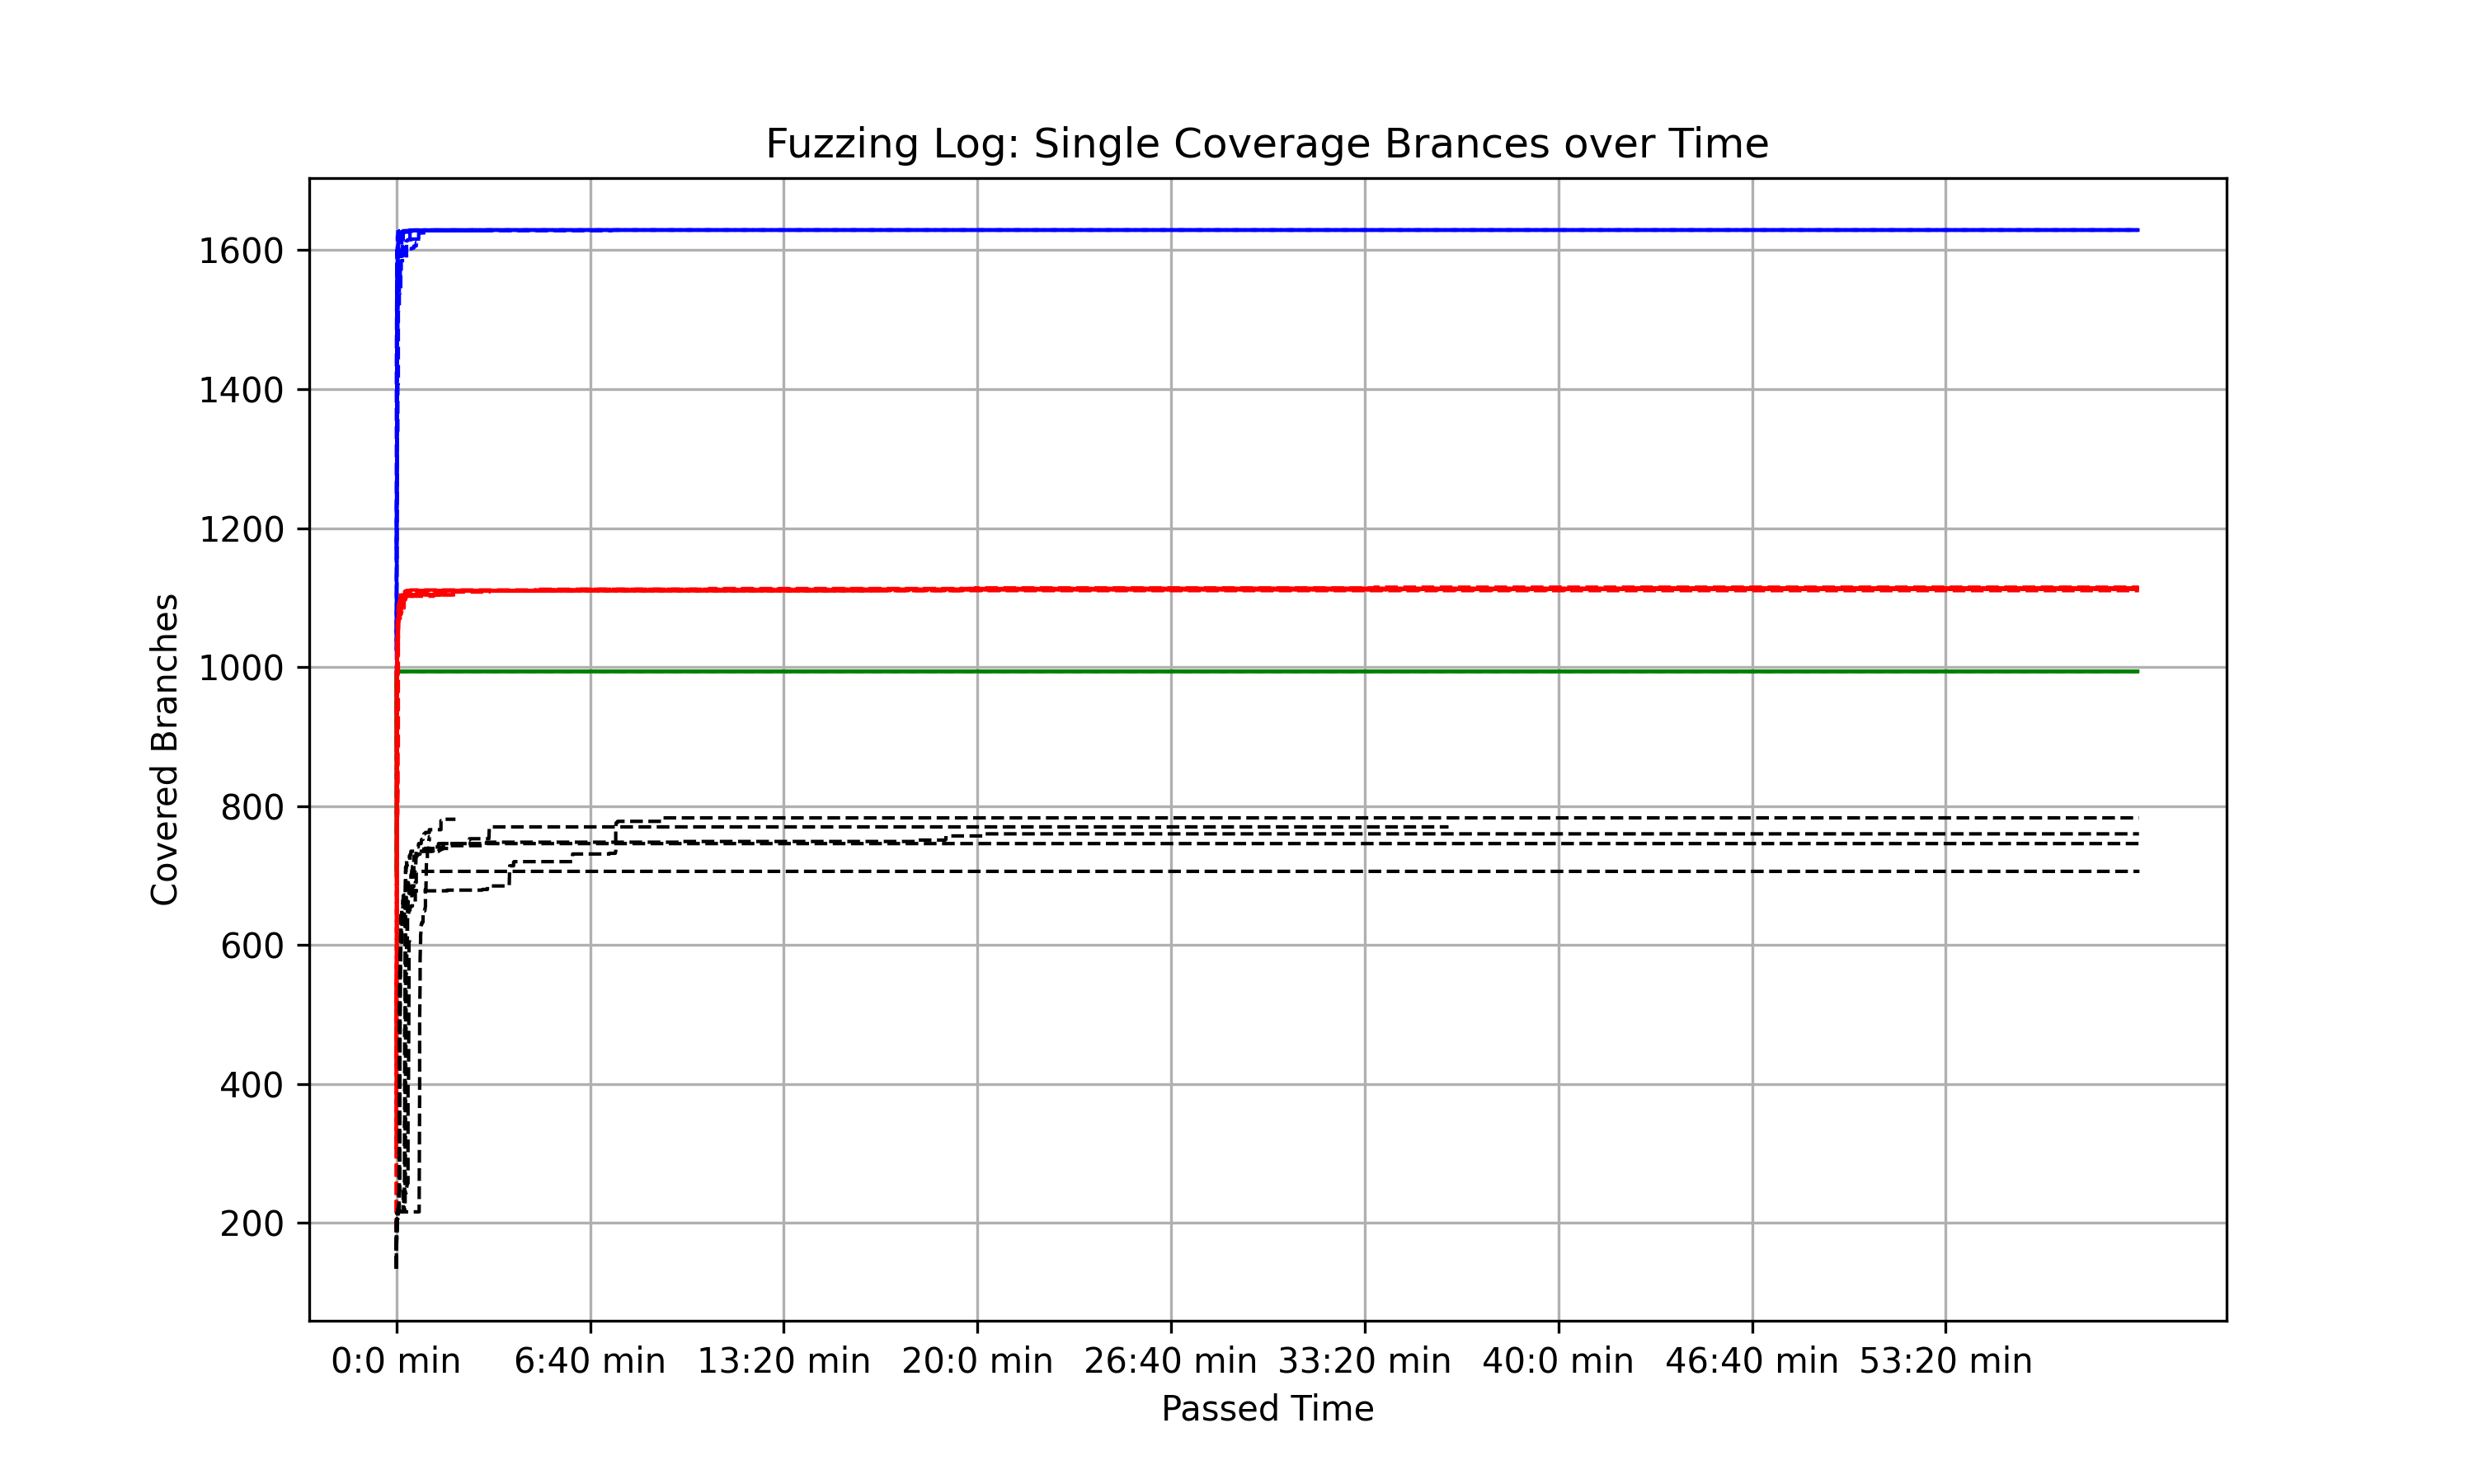
\includegraphics[width=\textwidth]{img/complete_coverage}
\captionof{figure}{Coverage for each repetition over time}\label{fig1}
\end{center}
\begin{center}
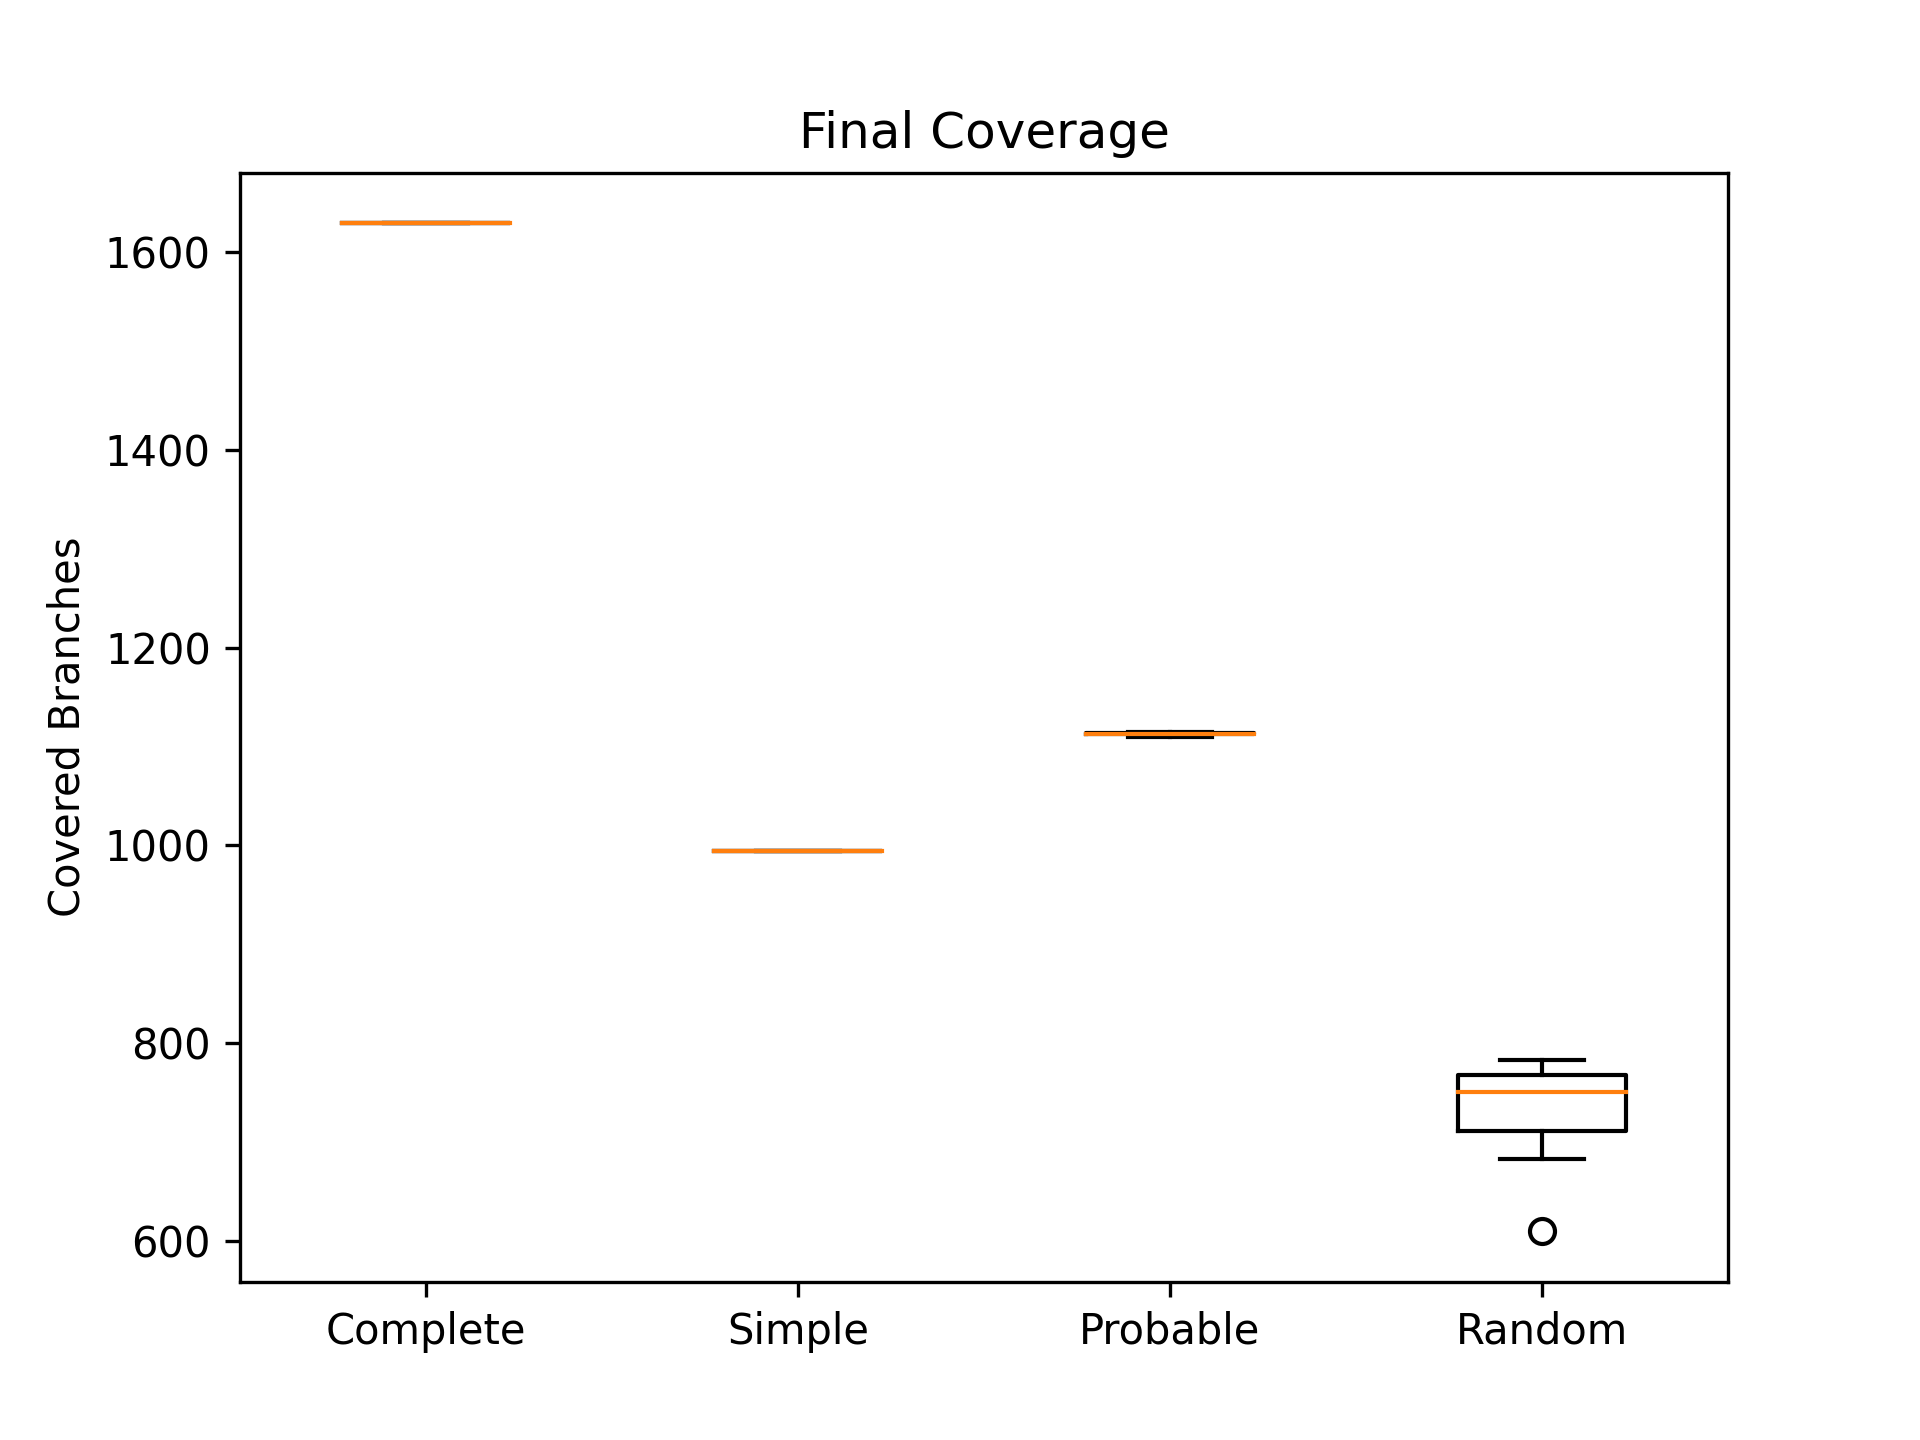
\includegraphics[width=\textwidth]{img/boxplot_coverage}
\captionof{figure}{Final Coverage}\label{fig2}
\end{center}

With our Complete Fuzzer, we managed to cover 1629 branches in every repetition. The Probable Fuzzer covered an average of 1112.9 branches. The Simple Fuzzer covered 994 Branches in every repitition. And the Random Fuzzer covered an average of 732,2 branches.

The number of covered branches for the Complete Fuzzer and the Simple Fuzzer did not change during the runs. This is why Figure 2 does not show any variance in the final coverage. The coverage of the Probable Fuzzer fluctuated slightly between 1110 and 1115 branches during the test runs. The coverage of the Random Fuzzer varied significantly more from 610 to 783 branches.
It can also be observed that the fuzzers find a lot of new branches in the first minute and that the coverage almost stops to increase after that.

\bgroup
\def\arraystretch{1.5}
\setlength\tabcolsep{1.5ex}
\begin{table}[]
    \caption{Coverage for each fuzzer.}
    \label{tab3}
    \begin{center}
        \begin{tabular}{|l|l|l|}
            \hline
            \textbf{Fuzzer} & \textbf{Average coverage} & \textbf{Average valid coverage} \\ \hline \hline
            Complete Fuzzer & 1629                      & 1629                            \\ \hline
            Random Fuzzer   & 732.2                     & 0                               \\ \hline
            Probable Fuzzer & 1112.9                    & 1053                            \\ \hline
            Simple Fuzzer   & 994                       & 994                             \\ \hline
        
        \end{tabular}
    \end{center}
\end{table}
\egroup

\subsubsection{Valid Coverage}
\begin{center}
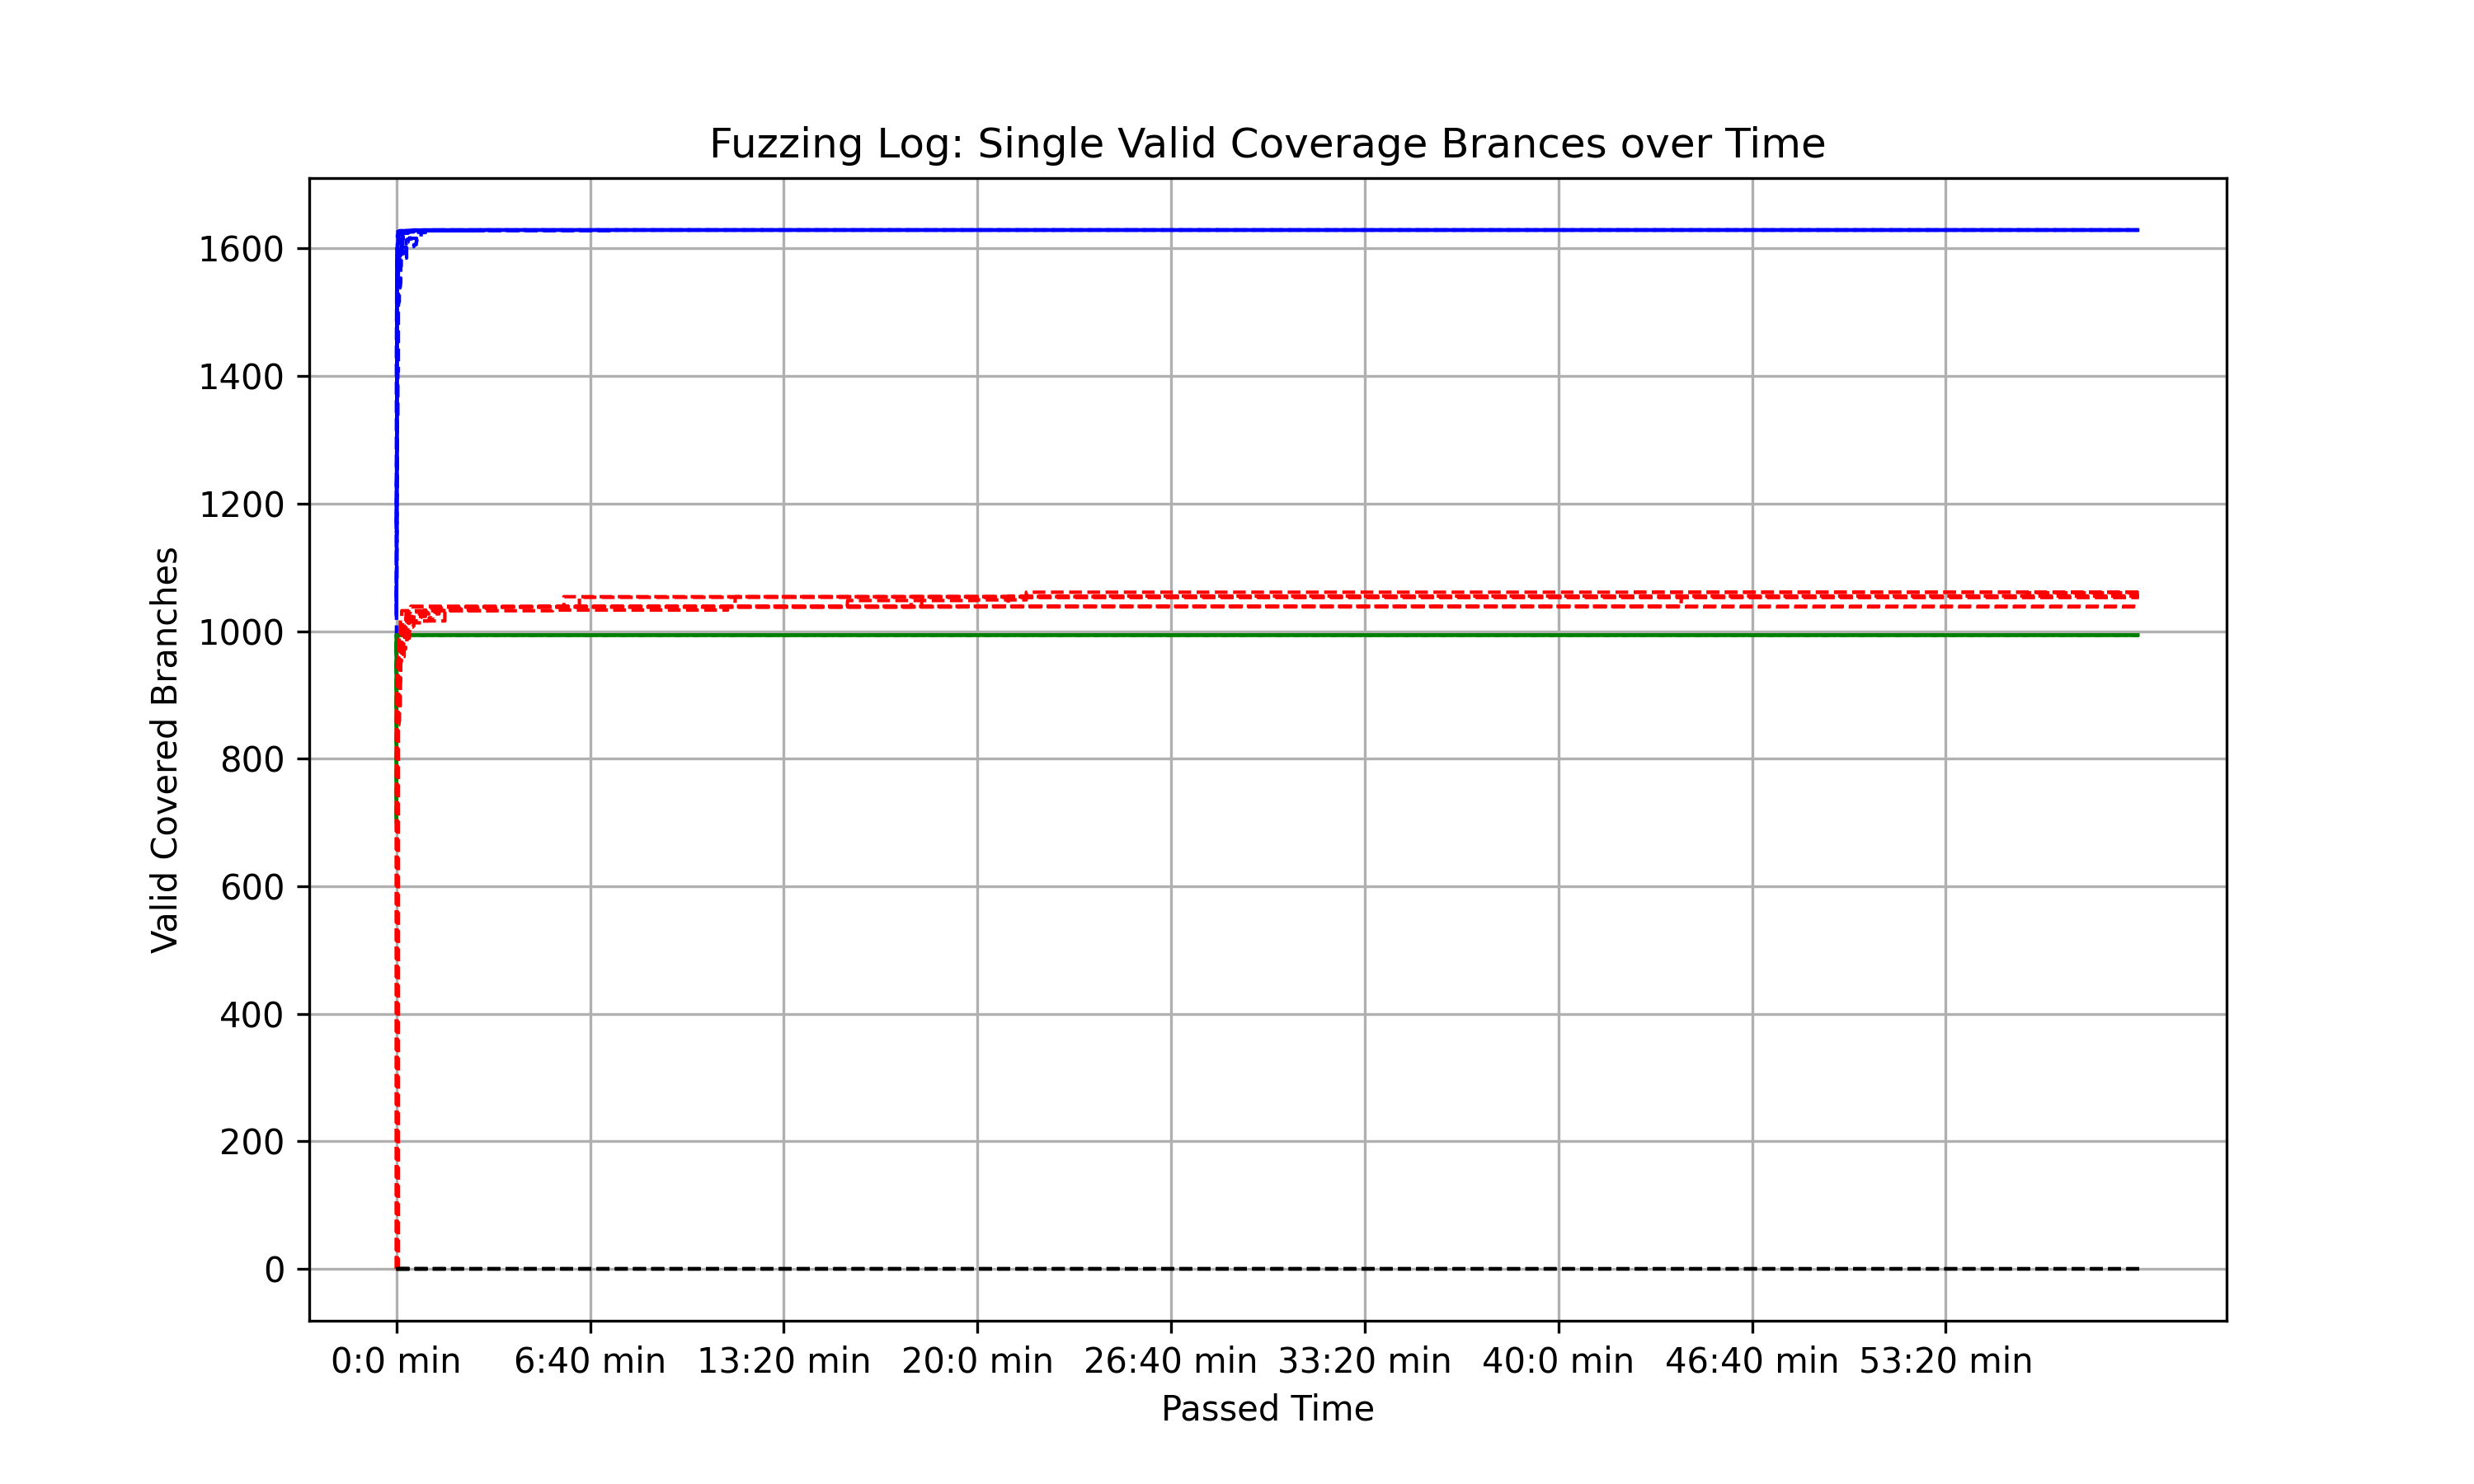
\includegraphics[width=\textwidth]{img/valid_coverage}
\captionof{figure}{Valid Coverage over time}\label{fig3}
\end{center}

\begin{center}
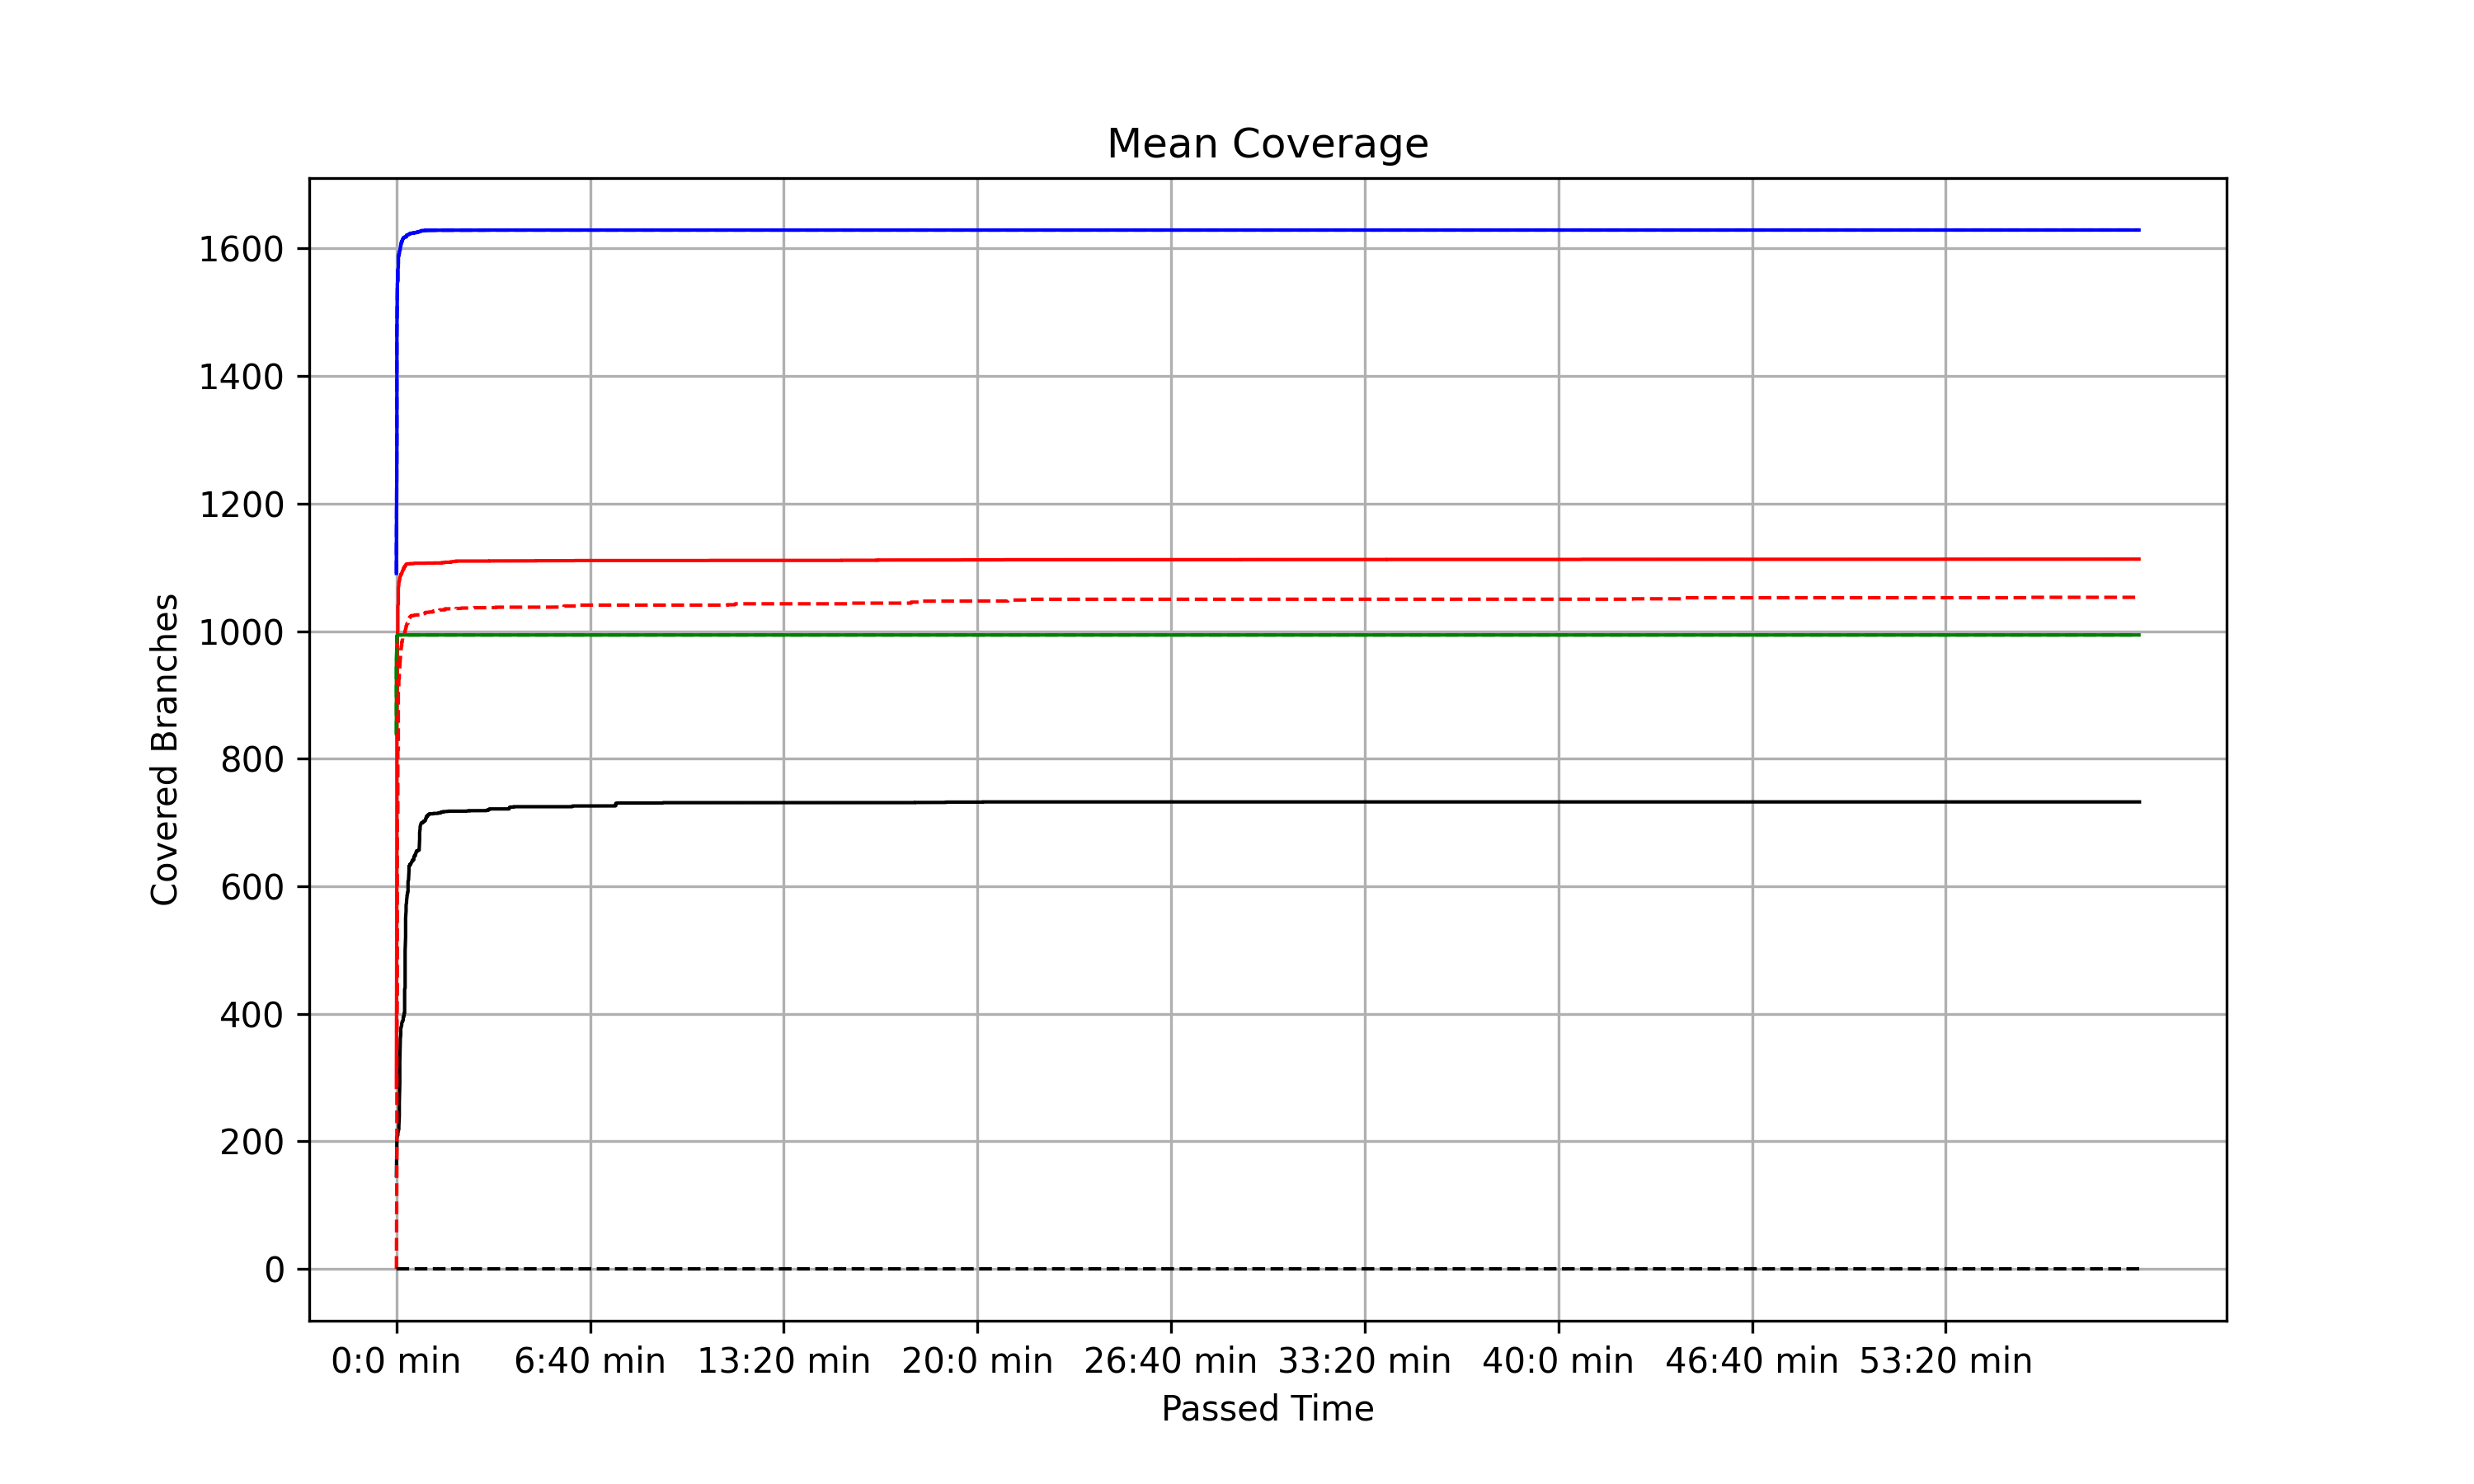
\includegraphics[width=\textwidth]{img/average_coverage}
\captionof{figure}{Mean Coverage over time (dotted graphs are valid coverage)}\label{fig4}
\end{center}
The valid coverage of the Complete Fuzzer and the Simple Fuzzer is identical to their total coverage. The Probable Fuzzer covers between 1038 and 1061 valid branches. That is slightly less than its total coverage. The Random Fuzzer had no valid coverage in our tests.

We checked the statistical significance of the differences in coverage using Mann-Whitney U tests. However, it is already clear from the figures that there is no overlap between the measurements of the fuzzers and that the differences are therefore significant.

\section{Result Discussion}
%TODO: Versucht die Ergebnisse der Experimente zu interpretieren und zu erklären (discussion). Zieht Sie Folgerungen aus den Ergebnissen (conclusion). Beschreibt die nächsten Schritte, die durchgeführt werden müssten/könnten/sollten (future work).
\subsection{Discussion}
As expected, the Complete Fuzzer provides the greatest coverage. As it contains many optional chunks and features, it can utilise many of PNGJ's functions. This becomes particularly clear when it is compared with the Simple Fuzzer, which covers a much smaller number of branches due to its limited options. The Probable Fuzzer has decent coverage for its relatively low implementation effort. However, due to the complexity of a PNG file, it is very unlikely to randomly generate one of the options that would enable even higher coverage. The same applies to the Random Fuzzer.

The fact that the fuzzers reach their maximum coverage after about a minute may be explained by the limited complexity of the PNGJ library as well as our test driver. The final coverage of the Probable and Random Fuzzers varies between runs, as sometimes options are found randomly that lead to more coverage and sometimes not. With the Complete and Simple Fuzzer, on the other hand, the structure is more strictly predefined, so it is more likely to generate all possible options, which seems to have happened during our runs.

When testing the Random Fuzzer, a Heap Error sometimes occurred which caused our fuzzing run to crash. We have not yet been able to find the cause of this error.

The valid coverage of the Complete Fuzzer and the Simple Fuzzer is identical to their total coverage, because these two Fuzzers only generate valid PNG-files. The valid coverage of the Probable Fuzzer is on average slightly below its total coverage, which should be due to the fact that this fuzzer can generate all critical chunks correctly. The random fuzzer has no valid coverage, as it is very unlikely to generate a correct PNG file at random.

\subsection{Conclusion}
Our generator creates valid PNG files that can contain all critical and optional chunks. This gives us significantly higher total and valid coverage on our fuzzing targets than simpler fuzzers. PNG is a relatively complex file format in which there are many dependencies between individual components. Therefore, a PNG generator needs a fairly fixed structure to generate valid files. Generating PNGs is thus not efficient with simple fuzzers that are largely based on chance.

\subsection{Future Work}
Our generator could be tested on other more complex fuzzing targets. In addition, the JQF guidance could be adapted to possibly deliver better results with our generator.

%
% ---- Bibliography ----
%
% BibTeX users should specify bibliography style 'splncs04'.
% References will then be sorted and formatted in the correct style.
%
% \bibliographystyle{splncs04}
% \bibliography{mybibliography}
%
\begin{thebibliography}{8}
\bibitem{PNG_specification}
Thomas Boutell. 1997. RFC Editor, PNG (Portable Network Graphics) Specification Version 1.0
\bibitem{security}
Libpng, Security vulnerabilities, CVEs,

\url{https://www.cvedetails.com/vulnerability-list/vendor\_id-7294/Libpng.html?page=1\&order=3\&trc=47\&sha=20a26d14531b8eff223b0769a2834502ea917ecf}
\bibitem{libpng_rationale}
Libpng, Rationale,
\url{http://www.libpng.org/pub/png/spec/1.2/PNG-Rationale.html}
\bibitem{JQF_paper}
Rohan Padhye, Caroline Lemieux, and Koushik Sen. 2019. JQF: Coverage-Guided Property-Based Testing in Java. In Proceedings of the 28th ACM SIGSOFT International Symposium on Software Testing and Analysis (ISSTA ’19), July 15–19, 2019, Beijing, China. ACM, New York, NY, USA, 4 pages. \url{https://doi.org/10.1145/3293882.3339002}
\bibitem{zest_guidance}
Rohan Padhye, Caroline Lemieux, Koushik Sen, Mike Papadakis, and Yves Le Traon. 2019. Semantic Fuzzing with Zest. In Proceedings of the 28th ACM SIGSOFT International Symposium on Software Testing and Analysis (ISSTA’19), July 15–19, 2019, Beijing, China. ACM, New York, NY, USA, 12 pages. \url{https://doi.org/10.1145/3293882.3330576}
\bibitem{PNGJ_github}
PNGJ GitHub-Page, \url{https://github.com/leonbloy/pngj?tab=readme-ov-file}
\bibitem{PNGJ_samples}
PNGJ Samples, 

\url{https://github.com/leonbloy/pngj/tree/master/src/test/java/ar/com/hjg/pngj/samples}
\bibitem{rfc_deflate_compression}
RFC 1951, Deflate Compressed Data Format Specification,

\url{https://datatracker.ietf.org/doc/html/rfc1951}
\bibitem{java_util_zip_docs}
Package \texttt{java.util.zip},

\url{https://download.java.net/java/early\_access/valhalla/docs/api/java.base/java/util/zip/package-summary.html}
\bibitem{libpng_file_structure}
Libpng: File structure,

\url{http://www.libpng.org/pub/png/spec/1.2/PNG-Structure.html}
\bibitem{libpng_chunks}
Libpng: Chunk specification, 

\url{http://www.libpng.org/pub/png/spec/1.2/PNG-Chunks.html}
\bibitem{libpng_deflate}
Libpng: Deflate algorithm,

\url{http://www.libpng.org/pub/png/spec/1.2/PNG-Compression.html}
\bibitem{libpng_filtering}
Libpng: Filtering,

\url{http://www.libpng.org/pub/png/spec/1.2/PNG-Filters.html}
\bibitem{libpng_data_representation}
Libpng: Data representation,

\url{http://www.libpng.org/pub/png/spec/1.2/PNG-DataRep.html}
\end{thebibliography}
\end{document}
